\documentclass[12pt, openany]{report}
\usepackage[utf8]{inputenc}
\usepackage[T1]{fontenc}
\usepackage[a4paper,left=2cm,right=2cm,top=2cm,bottom=2cm]{geometry}
\usepackage[french]{babel}
\usepackage[pdftex]{graphicx}
\usepackage{enumitem}
\usepackage{array}
\usepackage{pdfpages}

\setlength{\parindent}{0cm}
\setlength{\parskip}{1ex plus 0.5ex minus 0.2ex}
\newcommand{\hsp}{\hspace{20pt}}
\newcommand{\HRule}{\rule{\linewidth}{0.5mm}}
\newcolumntype{M}[1]{>{\centering\arraybackslash}m{#1}}

\begin{document}
    \begin{titlepage}
        \begin{center}
            \textsc{\LARGE École Polytechnique de l'Université de Tours}
            \\[2cm]

            
\includegraphics{img/polytech}
            \\[2cm]

            \HRule \\[0.4cm]
            { \huge \bfseries Carnet de suivi\\[0.4cm] }

            \HRule \\[2cm]

            \begin{minipage}{0.4\textwidth}
                \begin{flushleft} \large
\textsc{Brouard} Romain\\\end{flushleft}
            \end{minipage}
            \begin{minipage}{0.4\textwidth}
                \begin{flushright} \large
\emph{Tutrice académique:}\\ Mme. \textsc{Rault} Tiffen\\
\emph{Maître d'apprentissage:}\\ M. \textsc{Berruer} Stéphane\\
\end{flushright}
            \end{minipage}

            \vfill

            {\large 1\ier{} Septembre 2023 — 31 Août 2023}


\includegraphics[width=\textwidth]{/home/romain/Bureau/Suivi/carnet-de-suivi/test/eiffage.png}


        \end{center}
    \end{titlepage}

    \setcounter{tocdepth}{1}
    \tableofcontents

    \chapter{Présentation}
\section*{Semaine 36}
\begin{tabular}{|l|l|l|l|}
\hline
Matière & Description & Evaluation & Commentaire \\ 
\hline
Remise à niveau mathématique & - Cours, sur les fonctions usuelles & O (Sans Objet) & A VOUS DE LE REMPLIR - NE RIEN ÉCRIRE - MERCI \\ 
\hline
Remise à niveau mathématique & - TD sur les fonctions usuelles & O (Sans Objet) & A VOUS DE LE REMPLIR - NE RIEN ÉCRIRE - MERCI \\ 
\hline
Projet Accueil & "- Présentation du projet d'accueil- Qu'est ce que l'innovation?- Des intervenants nous ont présentés quelques exemples d'innovations" & O (Sans Objet) & A VOUS DE LE REMPLIR - NE RIEN ÉCRIRE - MERCI \\ 
\hline
Fresque du climat & - Réalisation d'une fresque du climat avec notre groupe de projet d'accueil & O (Sans Objet) & A VOUS DE LE REMPLIR - NE RIEN ÉCRIRE - MERCI \\ 
\hline
Réunion de rentrée  & "- Réunion de rentrée POLYTECH- Présentation de la formation par apprentissage" & O (Sans Objet) & A VOUS DE LE REMPLIR - NE RIEN ÉCRIRE - MERCI \\ 
\hline
Réunion & - Réunion de rentrée BDE & O (Sans Objet) & A VOUS DE LE REMPLIR - NE RIEN ÉCRIRE - MERCI \\ 
\hline
TOEIC & - Test du TOEIC & O (Sans Objet) & A VOUS DE LE REMPLIR - NE RIEN ÉCRIRE - MERCI \\ 
\hline
Réunion & - Présentation de l'ENT & O (Sans Objet) & A VOUS DE LE REMPLIR - NE RIEN ÉCRIRE - MERCI \\ 
\hline
\end{tabular}

\section*{Semaine 37}
\begin{tabular}{|l|l|l|l|}
\hline
Matière & Description & Evaluation & Commentaire \\ 
\hline
Remise à niveau mathématique & "- Cours sur les nombres complexes- TD sur les nombres complexes" & O (Sans Objet) & A VOUS DE LE REMPLIR - NE RIEN ÉCRIRE - MERCI \\ 
\hline
Anglais & "- Presentation du programme - Cours à l'oral" & O (Sans Objet) & A VOUS DE LE REMPLIR - NE RIEN ÉCRIRE - MERCI \\ 
\hline
Automatisme & - Introduction à l'automatisme & O (Sans Objet) & A VOUS DE LE REMPLIR - NE RIEN ÉCRIRE - MERCI \\ 
\hline
Remise à niveau informatique & - Cours sur l'histoire et le fonctionnement d'Unix et de bash & O (Sans Objet) & A VOUS DE LE REMPLIR - NE RIEN ÉCRIRE - MERCI \\ 
\hline
Remise à niveau électronique & - Cours d'introduction & O (Sans Objet) & A VOUS DE LE REMPLIR - NE RIEN ÉCRIRE - MERCI \\ 
\hline
Projet Accueil & - Prise de connaisance du projet interspecialités & O (Sans Objet) & A VOUS DE LE REMPLIR - NE RIEN ÉCRIRE - MERCI \\ 
\hline
\end{tabular}

\section*{Semaine 38}
\begin{tabular}{|l|l|l|l|}
\hline
Matière & Description & Evaluation & Commentaire \\ 
\hline
Remise à niveau informatique & - TP de remise à niveau où chaqun avance à son rythme & O (Sans Objet) & A VOUS DE LE REMPLIR - NE RIEN ÉCRIRE - MERCI \\ 
\hline
Anglais & "- Exposé sur un article choisi- Travail de discussion en petits groupe- Prise de note d'une vidéo" & O (Sans Objet) & A VOUS DE LE REMPLIR - NE RIEN ÉCRIRE - MERCI \\ 
\hline
Remise à niveau mathématique & "- Cours sur les nombres complexes- TD sur les nombres complexes" & O (Sans Objet) & A VOUS DE LE REMPLIR - NE RIEN ÉCRIRE - MERCI \\ 
\hline
Automatisme & "-Découverte Grafcet, Gemma" & O (Sans Objet) & A VOUS DE LE REMPLIR - NE RIEN ÉCRIRE - MERCI \\ 
\hline
Elections délégués & Antoine Balan et Alexandre Bourcier élus délégués & O (Sans Objet) & A VOUS DE LE REMPLIR - NE RIEN ÉCRIRE - MERCI \\ 
\hline
AMIIC & "-Découverte diagramme bête à cornes, schéma fonctionnel de niveau 1" & O (Sans Objet) & A VOUS DE LE REMPLIR - NE RIEN ÉCRIRE - MERCI \\ 
\hline
\end{tabular}

\section*{Semaine 41}
\begin{tabular}{|l|l|l|l|}
\hline
Matière & Description & Evaluation & Commentaire \\ 
\hline
Semaine internationale & "- Présentations mobilités internationales - Rencontres avec des étudiants étrangers" & O (Sans Objet) & A VOUS DE LE REMPLIR - NE RIEN ÉCRIRE - MERCI \\ 
\hline
Projet Accueil & "- Travail en autonomie sur le projet- Réunions pour aprofondir les differantes parties du projet" & O (Sans Objet) & A VOUS DE LE REMPLIR - NE RIEN ÉCRIRE - MERCI \\ 
\hline
Automatisme & "- CM sur la logique cablée- TD de mise en application des notions abordés en CM" & O (Sans Objet) & A VOUS DE LE REMPLIR - NE RIEN ÉCRIRE - MERCI \\ 
\hline
Anglais & "- Exposé sur un article choisi- Jeu de discussion par groupe de 3- Comprehension orale d'une vidéo- Evaluation de vocabulaire" & O (Sans Objet) & A VOUS DE LE REMPLIR - NE RIEN ÉCRIRE - MERCI \\ 
\hline
Remise à niveau informatique & - TP de remise à niveau où chaqun avance à son rythme & O (Sans Objet) & A VOUS DE LE REMPLIR - NE RIEN ÉCRIRE - MERCI \\ 
\hline
Remise à niveau mathématique & - TD sur les matrices & O (Sans Objet) & A VOUS DE LE REMPLIR - NE RIEN ÉCRIRE - MERCI \\ 
\hline
\end{tabular}

\section*{Semaine 42}
\begin{tabular}{|l|l|l|l|}
\hline
Matière & Description & Evaluation & Commentaire \\ 
\hline
Algèbre & - CM et TD sur les équations vectorielles & O (Sans Objet) & A VOUS DE LE REMPLIR - NE RIEN ÉCRIRE - MERCI \\ 
\hline
Anglais & "- Exposé sur un article choisi- Vidéo, vocabulaire et activités sur le biomimétisme" & O (Sans Objet) & A VOUS DE LE REMPLIR - NE RIEN ÉCRIRE - MERCI \\ 
\hline
Algorithmique & "- CM d'introduction au LDA et aux opérations algorithmiques- TD : Exercices basiques de LDA" & O (Sans Objet) & A VOUS DE LE REMPLIR - NE RIEN ÉCRIRE - MERCI \\ 
\hline
Remise à niveau informatique & "- TP de C, feuilles 1 et 2 d'exercices" & O (Sans Objet) & A VOUS DE LE REMPLIR - NE RIEN ÉCRIRE - MERCI \\ 
\hline
Automatisme & "- Fin de la feuille d'exercices sur les GRAFCETs et le GEMMA- Première séance de TP, attribution des équipes" & O (Sans Objet) & A VOUS DE LE REMPLIR - NE RIEN ÉCRIRE - MERCI \\ 
\hline
AMIIC & "- CM sur l'analyse fonctionnelle, présentation du système support- TD sur l'analyse fonctionnelle" & O (Sans Objet) & A VOUS DE LE REMPLIR - NE RIEN ÉCRIRE - MERCI \\ 
\hline
Fondamenteaux de l'économie & "- CM (niveaux d'économie, ressources, biens et services, agents économiques, secteurs d'activité & indicateurs économiques (PIB))" & O (Sans Objet) & A VOUS DE LE REMPLIR - NE RIEN ÉCRIRE - MERCI \\ 
\hline
\end{tabular}

\section*{Semaine 43}
\begin{tabular}{|l|l|l|l|}
\hline
Matière & Description & Evaluation & Commentaire \\ 
\hline
Algorithmique & - Cours sur la syntaxe de l'algorithmique & O (Sans Objet) & A VOUS DE LE REMPLIR - NE RIEN ÉCRIRE - MERCI \\ 
\hline
Anglais & "- Exposé sur un article choisi- Travail de discussion en petits groupe- Prise de note d'une vidéo" & O (Sans Objet) & A VOUS DE LE REMPLIR - NE RIEN ÉCRIRE - MERCI \\ 
\hline
Automatisme & - TP par binome sur divers exercices & O (Sans Objet) & A VOUS DE LE REMPLIR - NE RIEN ÉCRIRE - MERCI \\ 
\hline
Algèbre & "- TD, Divers exercices autour des thèmes abordés précédemment" & O (Sans Objet) & A VOUS DE LE REMPLIR - NE RIEN ÉCRIRE - MERCI \\ 
\hline
AMIIC & "- Analyse de signaux du SF1D- Passage par petits groupes pour présenter l'analyse d'un signal choisi" & O (Sans Objet) & A VOUS DE LE REMPLIR - NE RIEN ÉCRIRE - MERCI \\ 
\hline
Algorithmique & - Exercices d'introduction à l'algorithmique & O (Sans Objet) & A VOUS DE LE REMPLIR - NE RIEN ÉCRIRE - MERCI \\ 
\hline
Remise à niveau informatique & - Dernier TP pour finir les feuilles d'exercices & O (Sans Objet) & A VOUS DE LE REMPLIR - NE RIEN ÉCRIRE - MERCI \\ 
\hline
AMIIC & - Cours sur les capteurs et les spécificités & O (Sans Objet) & A VOUS DE LE REMPLIR - NE RIEN ÉCRIRE - MERCI \\ 
\hline
Remise à niveau électronique & - TP autours des portes NAND & O (Sans Objet) & A VOUS DE LE REMPLIR - NE RIEN ÉCRIRE - MERCI \\ 
\hline
Droit du travail et des affaires & "- Cours d'introduction au droit du travail et des affaires- Presentation de différents cas spécifiques" & O (Sans Objet) & A VOUS DE LE REMPLIR - NE RIEN ÉCRIRE - MERCI \\ 
\hline
Droit du travail et des affaires & "- Suite du cours précédent- Preparation à l'évaluation" & O (Sans Objet) & A VOUS DE LE REMPLIR - NE RIEN ÉCRIRE - MERCI \\ 
\hline
Projet Accueil & "- Présentation des soutenances devant un jury- Presentation devant les autres éléves pour les lauréats" & O (Sans Objet) & A VOUS DE LE REMPLIR - NE RIEN ÉCRIRE - MERCI \\ 
\hline
AMIIC & - TD sur l'analyse d'un capteur et simulation de son fonctionnement & O (Sans Objet) & A VOUS DE LE REMPLIR - NE RIEN ÉCRIRE - MERCI \\ 
\hline
Projet Accueil & - Conclusion du projet d'accueil et auto évaluation de nos compétences & O (Sans Objet) & A VOUS DE LE REMPLIR - NE RIEN ÉCRIRE - MERCI \\ 
\hline
Algorithmique & - Exercices d'algorithmique orientés autour des tableaux & O (Sans Objet) & A VOUS DE LE REMPLIR - NE RIEN ÉCRIRE - MERCI \\ 
\hline
\end{tabular}

\section*{Semaine 47}
\begin{tabular}{|l|l|l|l|}
\hline
Matière & Description & Evaluation & Commentaire \\ 
\hline
Algèbre & - CM sur la diagonalisation de matrices & O (Sans Objet) & A VOUS DE LE REMPLIR - NE RIEN ÉCRIRE - MERCI \\ 
\hline
Anglais & "- Presentation des exposés- Retour sur le travail à la maison- Evaluation de vocabulaire" & O (Sans Objet) & A VOUS DE LE REMPLIR - NE RIEN ÉCRIRE - MERCI \\ 
\hline
Algorithmique & - Dernière séance de TP & O (Sans Objet) & A VOUS DE LE REMPLIR - NE RIEN ÉCRIRE - MERCI \\ 
\hline
Analyse & - CMs sur les équations différentielles & O (Sans Objet) & A VOUS DE LE REMPLIR - NE RIEN ÉCRIRE - MERCI \\ 
\hline
AMIIC & -TP d'intégration de capteurs & O (Sans Objet) & A VOUS DE LE REMPLIR - NE RIEN ÉCRIRE - MERCI \\ 
\hline
Base de données et Conception & - CM sur le dictionnaire de données & O (Sans Objet) & A VOUS DE LE REMPLIR - NE RIEN ÉCRIRE - MERCI \\ 
\hline
Fondamenteaux de l'économie & "- CM sur la formation des prix, l'inflation et le pouvoir d'achat" & O (Sans Objet) & A VOUS DE LE REMPLIR - NE RIEN ÉCRIRE - MERCI \\ 
\hline
Probabilités & - Professeur absent & O (Sans Objet) & A VOUS DE LE REMPLIR - NE RIEN ÉCRIRE - MERCI \\ 
\hline
\end{tabular}

\section*{Semaine 48}
\begin{tabular}{|l|l|l|l|}
\hline
Matière & Description & Evaluation & Commentaire \\ 
\hline
Analyse & - TD sur la dérivation et l'intégration & O (Sans Objet) & A VOUS DE LE REMPLIR - NE RIEN ÉCRIRE - MERCI \\ 
\hline
Anglais & "- Exposé sur un article choisi- Retour sur les activités réalisées au CRL- Quiz en interaction sur les inventions" & O (Sans Objet) & A VOUS DE LE REMPLIR - NE RIEN ÉCRIRE - MERCI \\ 
\hline
Prévention mal-être étudiant & - C'était très bien & O (Sans Objet) & A VOUS DE LE REMPLIR - NE RIEN ÉCRIRE - MERCI \\ 
\hline
Projet électronique & - Lancement des projets  & O (Sans Objet) & A VOUS DE LE REMPLIR - NE RIEN ÉCRIRE - MERCI \\ 
\hline
Probabilités & - CM introductif sur les probabilités conditionnelles & O (Sans Objet) & A VOUS DE LE REMPLIR - NE RIEN ÉCRIRE - MERCI \\ 
\hline
AMIIC & "- CM sur la fonction amplification- TD sur la Conversion Analogique-Numérique et les bases de la fonction amplification" & O (Sans Objet) & A VOUS DE LE REMPLIR - NE RIEN ÉCRIRE - MERCI \\ 
\hline
Algèbre & - TD sur la diagonalisation & O (Sans Objet) & A VOUS DE LE REMPLIR - NE RIEN ÉCRIRE - MERCI \\ 
\hline
Algorithmique & - TD sur les algorithmes de tri & O (Sans Objet) & A VOUS DE LE REMPLIR - NE RIEN ÉCRIRE - MERCI \\ 
\hline
Base de données et Conception & "- Notions de dépendences fonctionnelles et graphes de dépendences fonctionnelles- MCD et cardinalités" & O (Sans Objet) & A VOUS DE LE REMPLIR - NE RIEN ÉCRIRE - MERCI \\ 
\hline
Ordres de grandeur T.E.S & - Notions d'écologie et sensibilisation au réchauffement climatique & O (Sans Objet) & A VOUS DE LE REMPLIR - NE RIEN ÉCRIRE - MERCI \\ 
\hline
Langage C & "- CMs introductifs (types, opérations de base, etc.)" & O (Sans Objet) & A VOUS DE LE REMPLIR - NE RIEN ÉCRIRE - MERC \\ 
\hline
\end{tabular}

\chapter{Annexes}
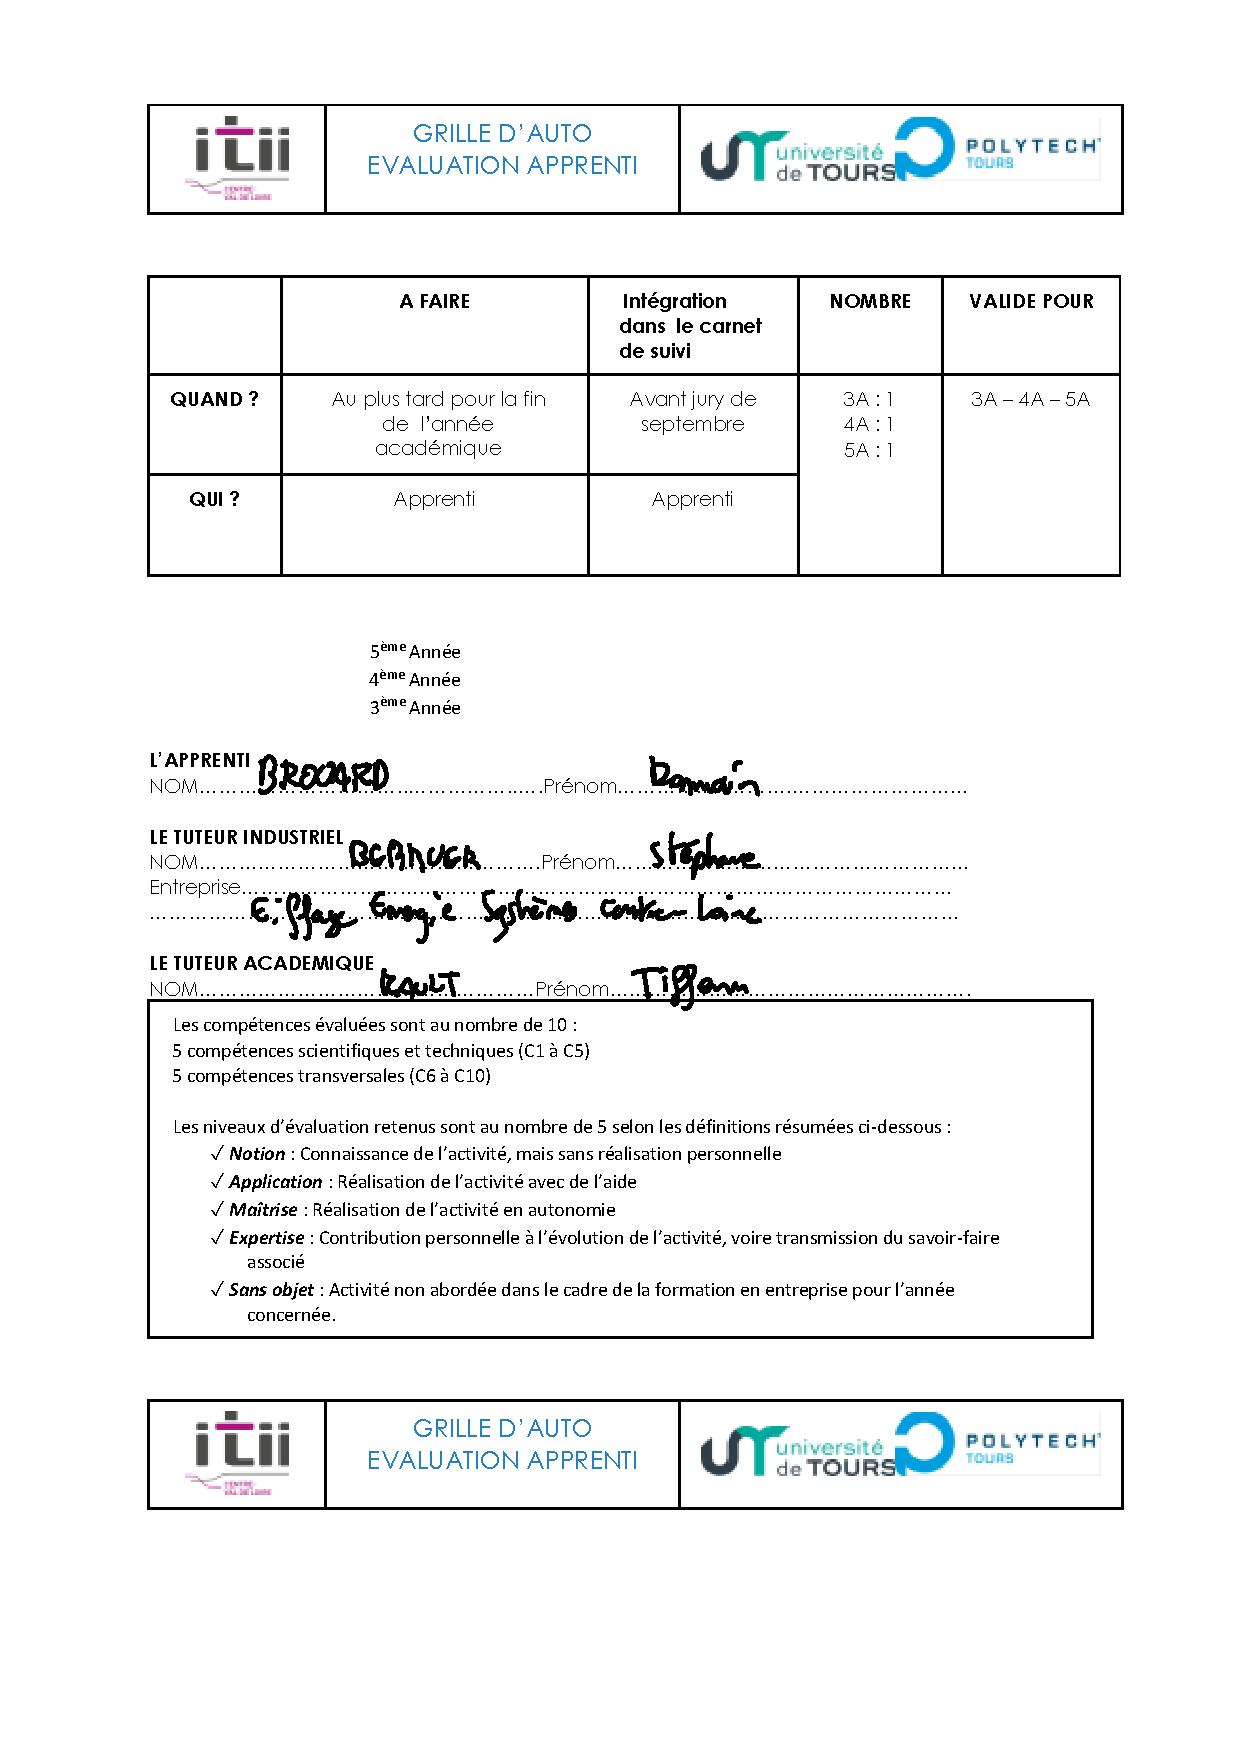
\includepdf[pages=-]{/home/romain/Bureau/Suivi/carnet-de-suivi/test/annexes/auto_eval_test.pdf}
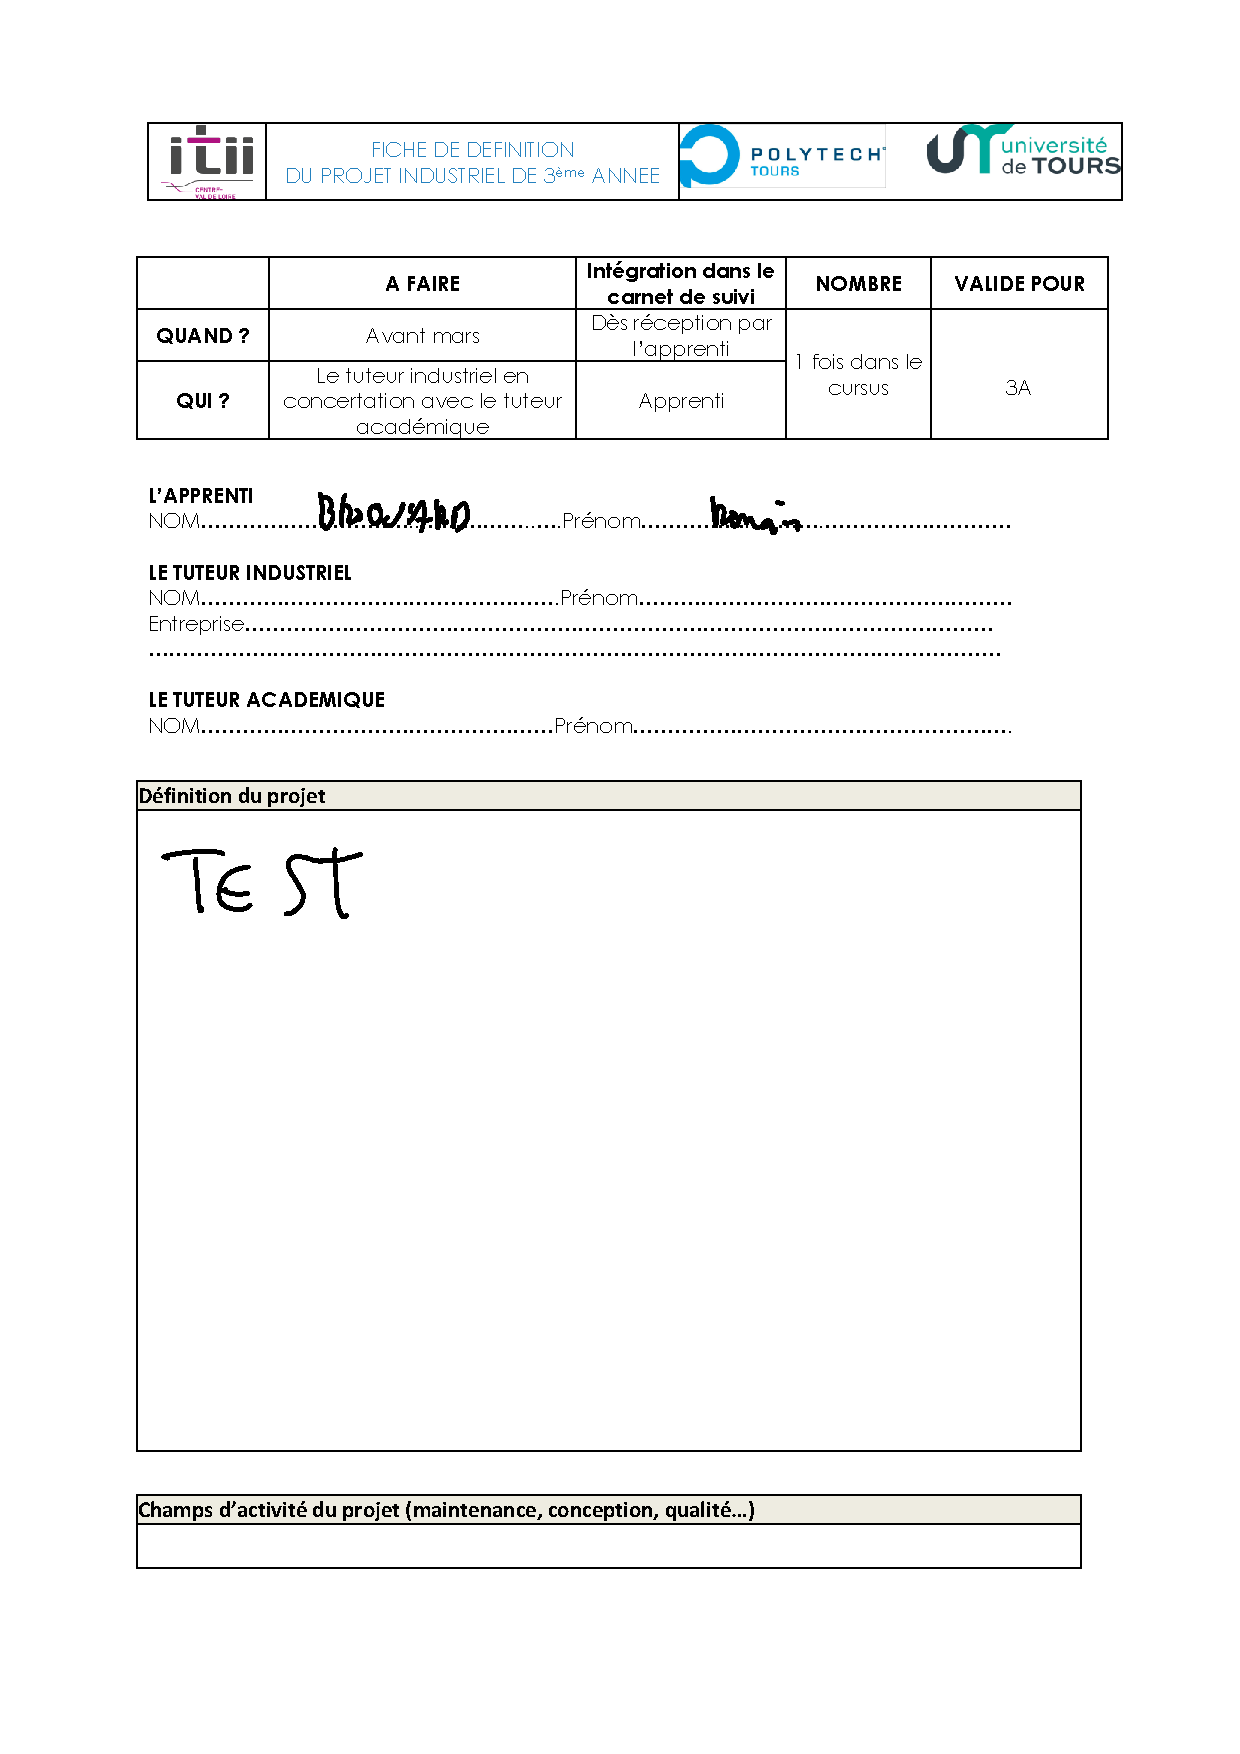
\includepdf[pages=-]{/home/romain/Bureau/Suivi/carnet-de-suivi/test/annexes/proj_indus_test.pdf}
\end{document}